\chapter{Praktische Anwendung von SHAP auf lineare Modelle}

In diesem Kapitel wird der Einsatz des SHAP-Frameworks zur Interpretation linearer Modelle im 
Kontext des maschinellen Lernens untersucht. Lineare Modelle, gekennzeichnet durch ihre Transparenz 
und einfache Struktur, bilden oft die Basis für das Verständnis komplexerer Algorithmen. 
Dennoch bleibt die Herausforderung bestehen, die Beiträge individueller Merkmale zur Modellvorhersage zu 
quantifizieren und zu interpretieren.

Die Anwendung von SHAP-Werten ermöglicht es, diesen Herausforderungen zu begegnen und Einblicke in 
die Modellvorhersagen zu gewähren, die über traditionelle Methoden hinausgehen. 
Dieses Kapitel führt in die Grundlagen des \textsf{shap}-Pakets ein, demonstriert dessen Anwendung auf einen 
spezifischen Datensatz und diskutiert die Berechnung sowie Interpretation der resultierenden SHAP-Werte.

\section{Lineare Modelle als analytische Grundlage}

In linearen Regressionsmodellen wird die Zielgröße als eine gewichtete Kombination der Eingangsmerkmale bestimmt. 
Die einfache lineare Struktur dieser Modelle erleichtert das Verständnis der Beziehungen zwischen den Eingangsdaten 
und den Vorhersagen. 

Lineare Modelle sind ein grundlegendes Werkzeug in der statistischen Modellierung und dienen dazu, das Verhältnis zwischen 
einer abhängigen Variablen, die üblicherweise mit $y^{(i)}$ bezeichnet wird, 
und einem oder mehreren Prädiktoren, den unabhängigen Variablen $x_i$, zu erfassen. 
Diese Beziehungen werden mittels linearer Gleichungen dargestellt, die für jede 
einzelne Beobachtung $i$ im Datensatz folgendermaßen formuliert werden können:

\begin{equation}
    y^{(i)} = \beta_0 + \sum_{j=1}^{p} \beta_j x^{(i)}_j + \epsilon^{(i)},
\label{eq:reg-model}
\end{equation}

wobei das Ergebnis, das von einem linearen Modell für eine gegebene Beobachtung vorhergesagt wird, sich als Summe der mit 
Gewichten $\beta_j$ versehenen Merkmale $p$ ergibt.

Hierbei stellt $y^{(i)}$ den beobachteten Wert der abhängigen Variablen für die Beobachtungseinheit
$i$ dar. Der Term $\beta_0$ ist der Achsenabschnitt oder y-Achsenabschnitt des Modells, 
welcher den erwarteten Wert von $y$ darstellt, wenn alle unabhängigen Variablen $x$ null sind. 
Die Summe $\sum_{j=1}^{p} \beta_j x^{(i)}_j$ berechnet sich aus den Produkten der Koeffizienten 
$\beta_j$ und den Werten der unabhängigen Variablen $x^{(i)}_j$ für jede Beobachtungseinheit $i$ 
und jeden Prädiktor $j$, wobei die Koeffizienten $\beta_j$ den geschätzten Einfluss der 
entsprechenden unabhängigen Variablen auf die abhängige Variable beschreiben.

Der Fehlerterm $\epsilon^{(i)}$ steht für die Residuen, also die Differenzen zwischen den beobachteten 
und durch das Modell geschätzten Werten von $y^{(i)}$. Es wird angenommen, dass diese Fehler normalverteilt sind, 
was bedeutet, dass Abweichungen in beiden Richtungen um den Mittelwert (hier null) 
mit abnehmender Wahrscheinlichkeit für größere Fehler auftreten \cite[S. 37]{Molnar_2022}.

In einem linearen Modell stellt der Achsenabschnitt die Basislinie dar, an der die Auswirkungen aller 
anderen Merkmale gemessen werden. Dieser Wert gibt an, was das Modell für die Zielvariable vorhersagen 
würde, wenn alle anderen Merkmale nicht vorhanden wären – der Ausgangspunkt der Vorhersage 
für einen Datensatz, in dem alle anderen Variablen auf null gesetzt sind. 
Es ist wichtig zu erwähnen, dass der Achsenabschnitt für sich genommen nicht immer eine praktische 
Bedeutung hat, da es selten vorkommt, dass alle Variablen tatsächlich den Wert null annehmen. 
Die wahre Aussagekraft des Achsenabschnitts tritt zutage, wenn die Daten so standardisiert wurden, 
dass ihre Mittelwerte bei null und die Standardabweichung bei eins liegen. Unter diesen Umständen repräsentiert der Achsenabschnitt 
die erwartete Zielvariable für einen hypothetischen Fall, in dem alle Merkmale ihren Durchschnittswert 
aufweisen \cite[S. 39]{Molnar_2022}.

Bei der Betrachtung einzelner Merkmale innerhalb des Modells sagt das Gewicht $\beta_j$ eines Merkmals, 
um wie viel sich die Zielvariable $y^{(i)}$ ändert, wenn das Merkmal $x^{(i)}_j$ um eine Einheit erhöht wird – und zwar unter 
der Annahme, dass alle anderen Merkmale unverändert bleiben. 
Dies ermöglicht es, den isolierten Effekt eines jeden Merkmals auf die Vorhersage zu verstehen \cite[S. 39]{Molnar_2022}.

Die optimalen Gewichte, oder Koeffizienten, eines linearen Regressionsmodells werden üblicherweise durch ein Verfahren bestimmt, 
das als Methode der kleinsten Quadrate (engl. \textit{Ordinary Least Squares}, OLS) bekannt ist. 
Diese Methode sucht die Koeffizienten \( \beta_0, \ldots, \beta_p \), welche die Summe der quadrierten 
Differenzen zwischen den beobachteten Werten der Zielvariablen \( y^{(i)} \) und den von dem Modell 
vorhergesagten Werten minimieren:

\begin{equation}
    \hat{\beta} = \arg \underset{\beta_0, \ldots, \beta_p}{\min} \ \sum_{i=1}^{n} \left( y^{(i)} - \left( \beta_0 + \sum_{j=1}^{p} \beta_j x_j^{(i)}\right)\right)^2.
\end{equation}

Das Ergebnis der Minimierung, \( \hat{\beta} \) stellt den Vektor der geschätzten Koeffizienten dar \cite[S. 37]{Molnar_2022}. 
In der vorliegenden Arbeit wird das Python-Paket \textsf{scikit-learn}\footnote{\url{https://scikit-learn.org}} verwendet, um die lineare Regression durchzuführen und die Koeffizienten 
\( \hat{\beta} \) zu bestimmen. 


\section{Einführung in das \textsf{shap} Python-Paket}
\label{sec:shap-package}

Das Python-Paket \textsf{shap}\footnote{\url{https://shap.readthedocs.io}} ist eine Open-Source-Bibliothek, die es Nutzern ermöglicht, 
die Auswirkungen von Merkmalen auf Vorhersagen von maschinellen Lernmodellen zu interpretieren und zu visualisieren. 
Entwickelt wurde die Bibliothek ursprünglich von Scott Lundberg und weiteren Mitwirkenden im Rahmen der Forschungsarbeit 
an der University of Washington \cite{NIPS2017_8a20a862}. Das Paket basiert auf dem Konzept der Shapley-Werte aus der kooperativen Spieltheorie 
und überträgt diese auf den Kontext des maschinellen Lernens, um als Tool für die Interpretierbarkeit und Erklärbarkeit 
von Modellvorhersagen zu dienen.

\urldef{\ploturl}\url{https://shap.readthedocs.io/en/latest/api.html#plots}

Die Kernfunktion des \textsf{shap}-Pakets ist die Berechnung von SHAP-Werten, welche die Auswirkung der 
Einzelmerkmale auf die Modellvorhersage quantifizieren. Jeder SHAP-Wert ist ein Maß dafür, wie viel jedes Merkmal 
zur Vorhersage beigetragen hat, im Vergleich zu einer durchschnittlichen Vorhersage über den gesamten Datensatz. 
Diese Werte sind besonders wertvoll, da sie ein Maß für die Bedeutung jedes Merkmals bieten. Diese Bedeutung kann 
sowohl lokal für einzelne Vorhersagen als auch global über das gesamte Modell interpretiert werden

Mit \textsf{shap} können Benutzer die Vorhersagen einer Vielzahl von Modellen interpretieren, 
von linearen Modellen bis hin zu komplexen Konstrukten wie tiefe neuronale Netzwerke. 
Die Bibliothek bietet eine vielseitige Auswahl an Visualisierungsoptionen, darunter Beeswarm-Plots, Dependence-Plots und 
Bar-Plots, die es ermöglichen, die SHAP-Werte intuitiv zu verstehen. Eine Übersicht aller Visualisierungsoptionen ist in der Dokumentation 
des Pakets zu finden\footnote{\ploturl}.
Diese Visualisierungen erleichtern es, Muster und Beiträge einzelner Merkmale zu erkennen, 
was nicht nur wertvolle Einblicke in die Leistung des Modells bietet, sondern auch zu faireren und transparenteren 
Modellentscheidungen führen kann. 

\urldef{\shapurl}\url{https://shap.readthedocs.io/en/latest/api.html#explainers}
\urldef{\exacturl}\url{https://github.com/shap/shap/blob/master/shap/explainers/_exact.py}

Im Kapitel \ref{subsec:linear-shap-estimator} wurde bereits der LinearExplainer aus dem \textsf{shap}-Paket 
vorgestellt, ein Beispiel für die verschiedenen Estimators, die das Paket in Form von Explainern bereitstellt. 
Das Paket bietet eine Vielzahl von Explainern, die auf unterschiedliche Modelltypen zugeschnitten sind. 
Einer der bemerkenswerten Aspekte von \textsf{shap} ist der auto Modus des Estimators, 
der automatisch den am besten geeigneten Explainer für das gegebene Modell auswählt. 
Diese Funktion ist besonders nützlich, da sie die Komplexität der Auswahl des richtigen Explainers 
reduziert und den Anwendungsprozess vereinfacht. Speziell für Modelle mit ca. 15 Merkmalen\footnote{\exacturl} wählt der 
auto Modus den exakten Explainer, der präzise SHAP-Werte auf Grundlage aller Daten und Koalitionen berechnet, was für Modelle mit einer geringeren Anzahl 
von Merkmalen effizient und praktikabel ist \cite[S. 40f]{Molnar_2023}. Eine Übersicht der zur Verfügung stehenden \textsf{shap}-Explainern ist in der
Dokumentation des Pakets zu finden\footnote{\shapurl}. 


\section{Einführung in den Datensatz}


Der Concrete Compressive Strength Datensatz ist eine umfassende Sammlung von Daten, 
die die Druckfestigkeit von Beton in Bezug auf verschiedene Bestandteile und das Alter des Betons untersucht. 
Die Bestandteile umfassen Zement, Hochofenschlacke, Flugasche, Wasser, Superplastifikator, 
groben Zuschlag und feinen Zuschlag \cite{misc_concrete_compressive_strength_165}.

\textbf{Ziel der Regression:} Das Ziel ist es, die Druckfestigkeit von Beton in Megapascal basierend 
auf seiner Zusammensetzung und dem Alter vorherzusagen. Diese Vorhersage ist entscheidend, 
da Beton das Fundament der modernen Welt bildet und seine Festigkeit für die Sicherheit und 
Langlebigkeit von Bauwerken von größter Bedeutung ist.

Der Datensatz umfasst folgende Variablen:

\begin{itemize}
    \item \textbf{cement (Zement)}: Menge an Zement (kg in einem m³ Gemisch). Zement ist ein Hauptbestandteil von Beton und wesentlich für dessen Festigkeit.
    \item \textbf{blast (Hochofenschlacke)}: Menge an Hochofenschlacke (kg in einem m³ Gemisch). Schlacke kann die Festigkeit und Haltbarkeit von Beton verbessern.
    \item \textbf{ash (Flugasche)}: Menge an Flugasche (kg in einem m³ Gemisch). Flugasche wird als Ersatz für Zement verwendet und beeinflusst die Verarbeitbarkeit und Festigkeit.
    \item \textbf{water (Wasser)}: Menge an Wasser (kg in einem m³ Gemisch). Wasser ist für die Hydratation des Zements und die Konsistenz des Betons notwendig.
    \item \textbf{superplasticizer (Superplastifikator)}: Menge an Superplastifikator (kg in einem m³ Gemisch). Superplastifikatoren verbessern die Fließfähigkeit und Verarbeitbarkeit von Beton.
    \item \textbf{coarse (Grober Zuschlag)}: Menge an grobem Zuschlag (kg in einem m³ Gemisch). Grober Zuschlag trägt zur Stabilität und Struktur des Betons bei.
    \item \textbf{fine (Feiner Zuschlag)}: Menge an feinem Zuschlag (kg in einem m³ Gemisch). Feiner Zuschlag beeinflusst die Dichte und die Oberflächeneigenschaften des Betons.
    \item \textbf{age (Alter)}: Alter des Betons in Tagen. Das Alter hat einen signifikanten Einfluss auf die Festigkeit des Betons.
    \item \textbf{strength (Druckfestigkeit)}: Die tatsächliche Druckfestigkeit von Beton (MPa). Dies ist die Zielvariable, die modelliert wird.
\end{itemize}
 
Die Bedeutung dieses Themas liegt in der zentralen Rolle, die Beton im Bauwesen spielt. 
Als eines der am meisten verwendeten Materialien weltweit, ist die genaue Vorhersage seiner Festigkeit von entscheidender 
Bedeutung für die Planung und den Bau sicherer und langlebiger Strukturen. Dieser Datensatz bietet daher wertvolle Einblicke für Ingenieure und Forscher, 
um die Eigenschaften und das Verhalten von Beton besser zu verstehen und zu optimieren.

\section{Explorative Datenanalyse \& Datenaufbereitung}

Der Datensatz wurde in Python mithilfe der Bibliothek \textsf{pandas} als \textsf{Dataframe} eingelesen.
Der vollständige Quellcode für das Einlesen der Daten sowie alle weiteren Analyseschritte ist 
im Anhang \ref{linreg} dieser Arbeit zu finden.

Tabelle \ref{tab:df-head} zeigt die ersten fünf Beobachtungen des Datensatzes:

\begin{table}[!h]
    \caption{Auszug aus dem Concrete Compressive Strength Datensatz.}
    \footnotesize
    \begin{tabularx}{\textwidth}{Xrrrrrrrrr}
    \toprule
    Index & \rotatebox{90}{cement} & \rotatebox{90}{blast} & \rotatebox{90}{ash} & \rotatebox{90}{water} & \rotatebox{90}{superplasticizer} & \rotatebox{90}{coarse} & \rotatebox{90}{fine} & \rotatebox{90}{age} & \rotatebox{90}{strength} \\
    \midrule
    0 & 540.0 & 0.0 & 0.0 & 162.0 & 2.5 & 1040.0 & 676.0 & 28 & 79.986111 \\
    1 & 540.0 & 0.0 & 0.0 & 162.0 & 2.5 & 1055.0 & 676.0 & 28 & 61.887366 \\
    2 & 332.5 & 142.5 & 0.0 & 228.0 & 0.0 & 932.0 & 594.0 & 270 & 40.269535 \\
    3 & 332.5 & 142.5 & 0.0 & 228.0 & 0.0 & 932.0 & 594.0 & 365 & 41.052780 \\
    4 & 198.6 & 132.4 & 0.0 & 192.0 & 0.0 & 978.4 & 825.5 & 360 & 44.296075 \\
    \bottomrule
    \end{tabularx}
    \label{tab:df-head}
    \normalsize\\
    Quelle: Eigene Darstellung, \ref{linreg}.
\end{table}

\begin{table}[!h]
    \caption{Statistische Übersicht des Concrete Compressive Strength Datensatzes.}
    \footnotesize
    \begin{tabularx}{\textwidth}{Xrrrrrrr}
    \toprule
    Variable & mean & std & min & 25\% & 50\% & 75\% & max \\
    \midrule
    cement & 278.629 & 104.345 & 102.0 & 190.68 & 265.0 & 349.0 & 540.0 \\
    blast & 72.043 & 86.171 & 0.0 & 0.0 & 20.0 & 142.5 & 359.4 \\
    ash & 55.535 & 64.207 & 0.0 & 0.0 & 0.0 & 118.27 & 200.1 \\
    water & 182.074 & 21.341 & 121.75 & 166.61 & 185.7 & 192.94 & 247.0 \\
    superplasticizer & 6.032 & 5.92 & 0.0 & 0.0 & 6.1 & 10.0 & 32.2 \\
    coarse & 974.376 & 77.58 & 801.0 & 932.0 & 968.0 & 1031.0 & 1145.0 \\
    fine & 772.687 & 80.34 & 594.0 & 724.3 & 780.0 & 822.2 & 992.6 \\
    age & 45.857 & 63.735 & 1.0 & 7.0 & 28.0 & 56.0 & 365.0 \\
    strength & 35.250 & 16.285 & 2.332 & 23.524 & 33.798 & 44.868 & 82.599 \\
    \bottomrule
    \end{tabularx}
    \label{tab:statistics}
    \normalsize
    \\ Quelle: Eigene Darstellung, \ref{linreg}.
\end{table}

Tabelle \ref{tab:statistics} offenbart eine signifikante Variabilität und Bandbreite 
in den Werten aller Variablen. Um eine gleichmäßige Verteilung zu erreichen und den 
Einfluss von Ausreißern zu verringern, werden die Daten einer logarithmischen Transformation unterzogen. 
Diese Methode dient dazu, die Skalierung der Variablen zu vereinheitlichen und ihre Verteilung zu normalsieren, 
was die Genauigkeit und Stabilität des Regressionsmodells verbessert.
Abbildung \ref{pic:box} zeigt einen Boxplot der jeweiligen Merkmale vor und 
nach der logarthimischen Transformation.

\begin{figure}[!h]
    \caption{Boxplot der Merkmale vor und nach der Log-Transformation.}
    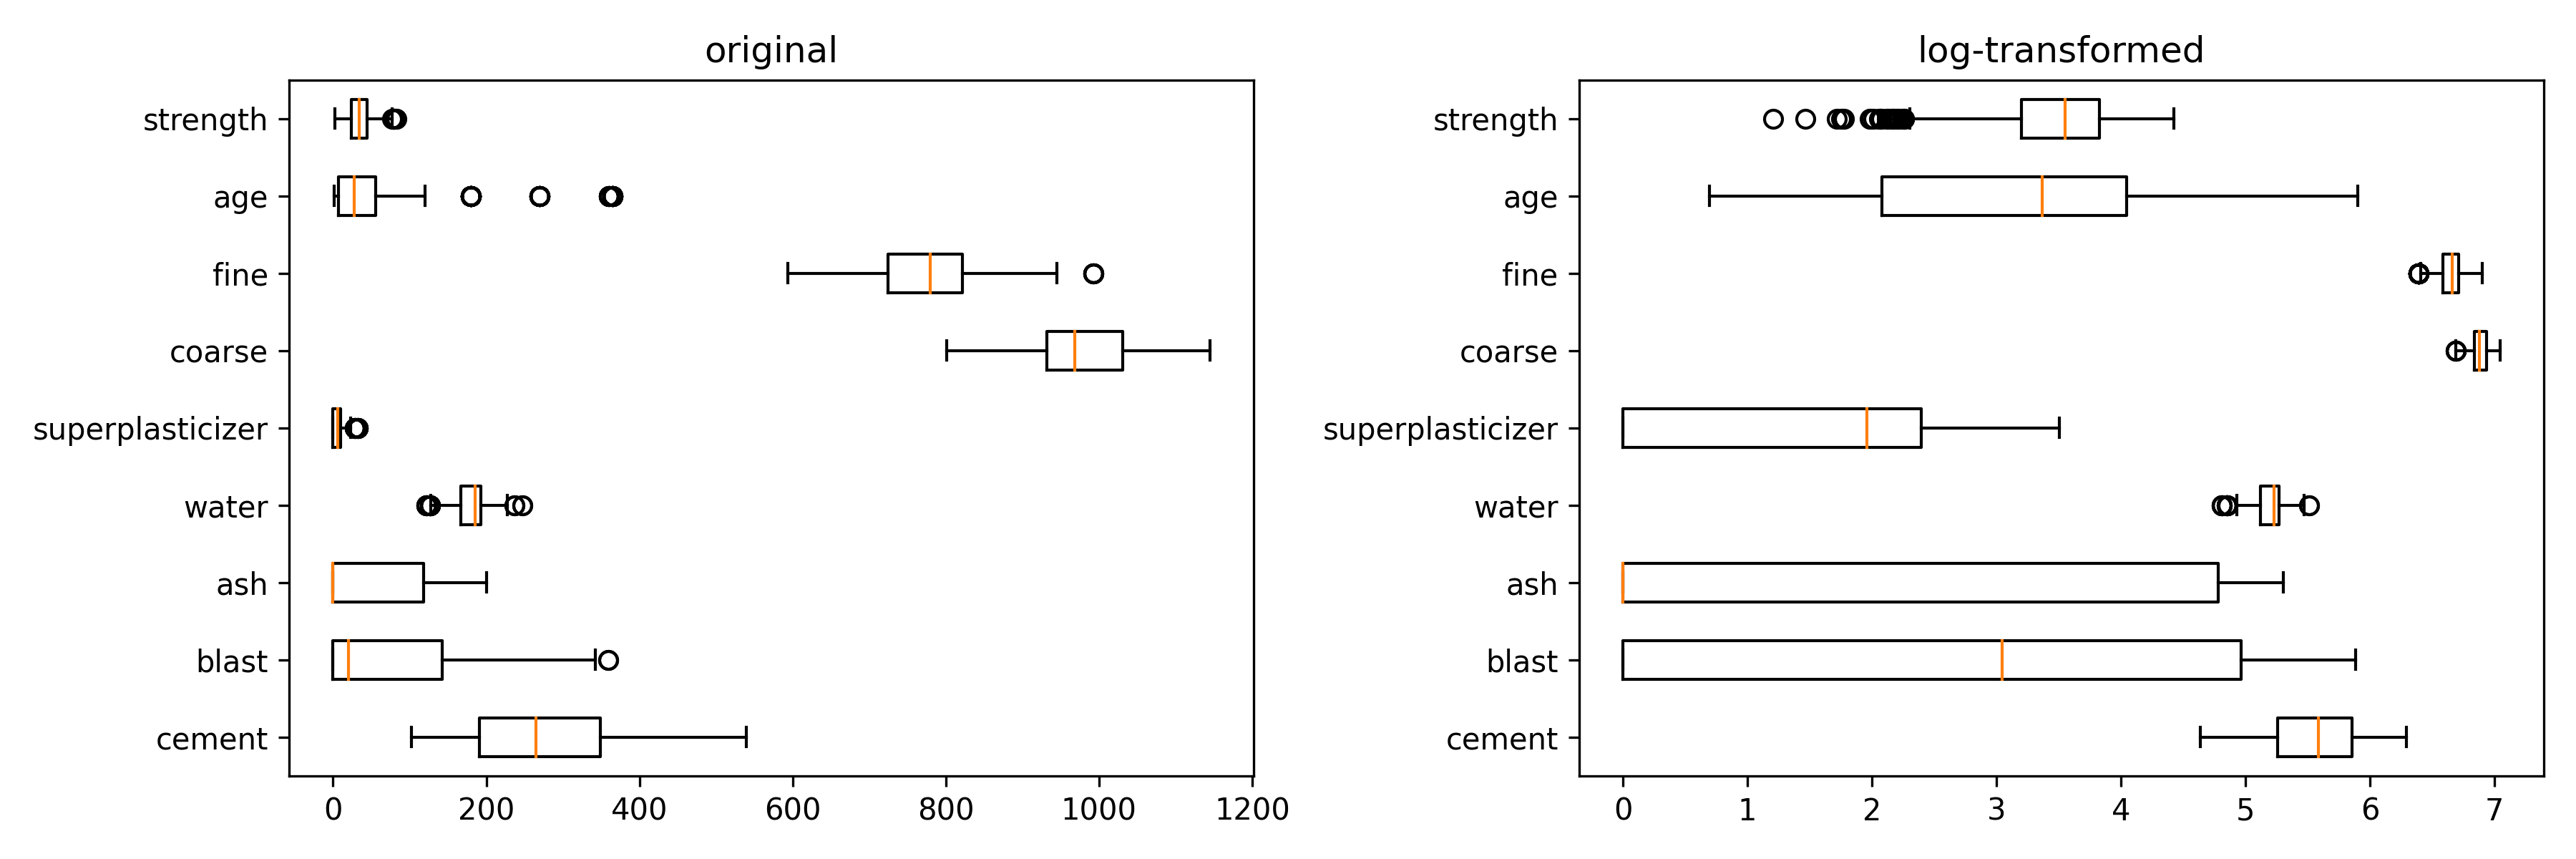
\includegraphics[width=1\textwidth]{../scripts/images/boxplot.png}
    Quelle: Eigene Darstellung, \ref{linreg}.
    \label{pic:box}
\end{figure}

In einem Boxplot zeigt die zentrale Box die Interquartilspanne (IQR), 
die die mittleren 50\% der Daten umfasst, mit dem unteren Rand als erstes Quartil 
(25\% der Daten darunter) und dem oberen Rand als drittes Quartil (75\% der Daten darunter). 
Der horizontale Strich in der Mitte ist der Median, der die Daten in zwei Hälften teilt. 
Die Whiskers, die Linien, welche von der Box ausgehen, stellen die Streuung außerhalb der Quartile dar und 
erstrecken sich normalerweise bis zu den äußersten regulären Datenpunkten. 
Datenpunkte außerhalb des Bereichs der Whiskers werden als Ausreißer betrachtet und separat markiert \cite[S. 43]{Molnar_2022}. 

Abbildung \ref{pic:hist} zeigt die Häufigkeitsverteilung aller Merkmale des Datensatzes 
nach der logarithmischen Transformation. 

\begin{figure}[!h]
    \caption{Verteilungen der Merkmale.}
    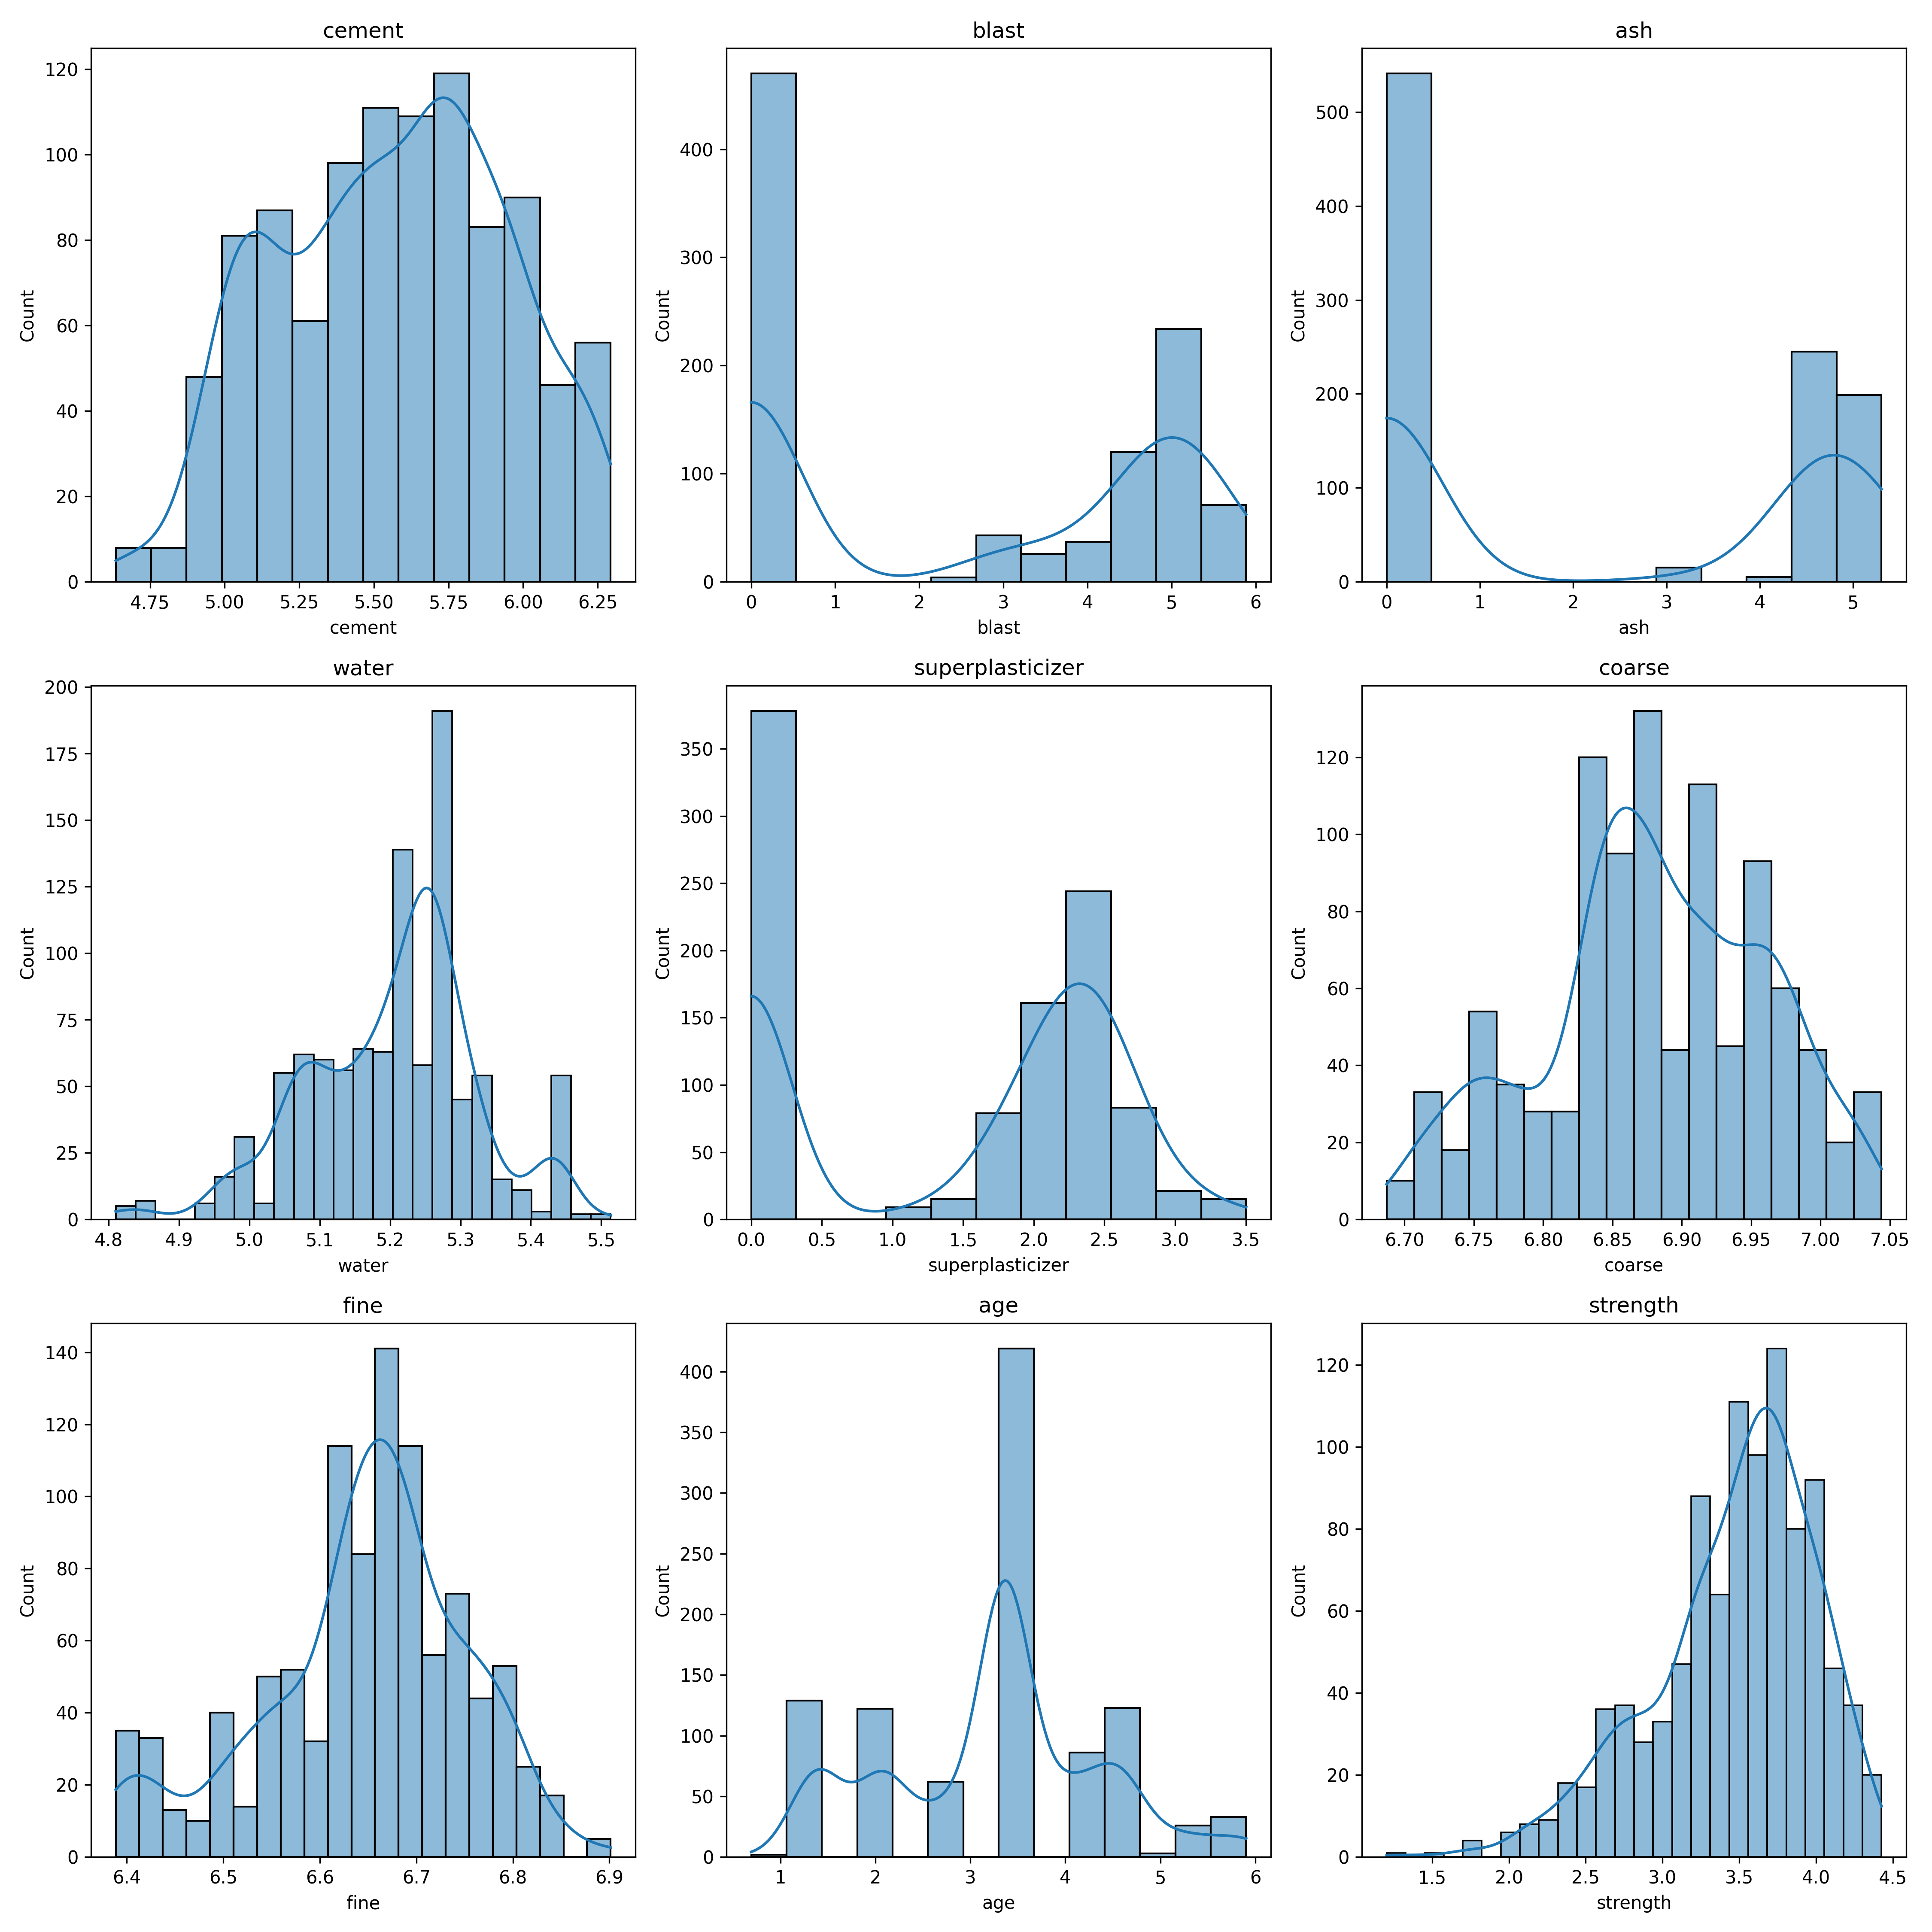
\includegraphics[width=1\textwidth]{../scripts/images/dist.png}
    Quelle: Eigene Darstellung, \ref{linreg}.
    \label{pic:hist}
\end{figure}

Die Korrelationsmatrix, dargestellt in Abbildung \ref{pic:corr}, 
quantifziert die Beziehungen zwischen den einzelnen Bestandteilen des Betons und der Zielvariablen der 
Betondruckfestigkeit. Die Koeffizienten bewegen sich zwischen -0.61 und 0.63, was auf 
unterschiedlich starke Korrelationen hinweist. Ein markantes Beispiel ist der positive Wert 
von 0.63 zwischen Asche und Wasser, was eine starke direkte Beziehung nahelegt, während der Wert 
von -0.61 zwischen Wasser und Superplastifikator auf eine starke umgekehrte Beziehung hindeutet. 
Die Zielvariable der Betondruckfestigkeit zeigt die stärkste direkte Korrelation mit dem Zementgehalt (0.46), 
was darauf schließen lässt, dass ein höherer Zementanteil tendenziell zu einer stärkeren Betonmischung führt. 
Diese Korrelationsmuster sind essentiell für die Modellentwicklung, da sie Aufschluss darüber geben, welche 
Mischungsbestandteile einen bedeutenden Einfluss auf die Betondruckfestigkeit haben könnten.

\begin{figure}[h]
    \caption{Korrelationsmatrix der Merkmale im Datensatz.}
    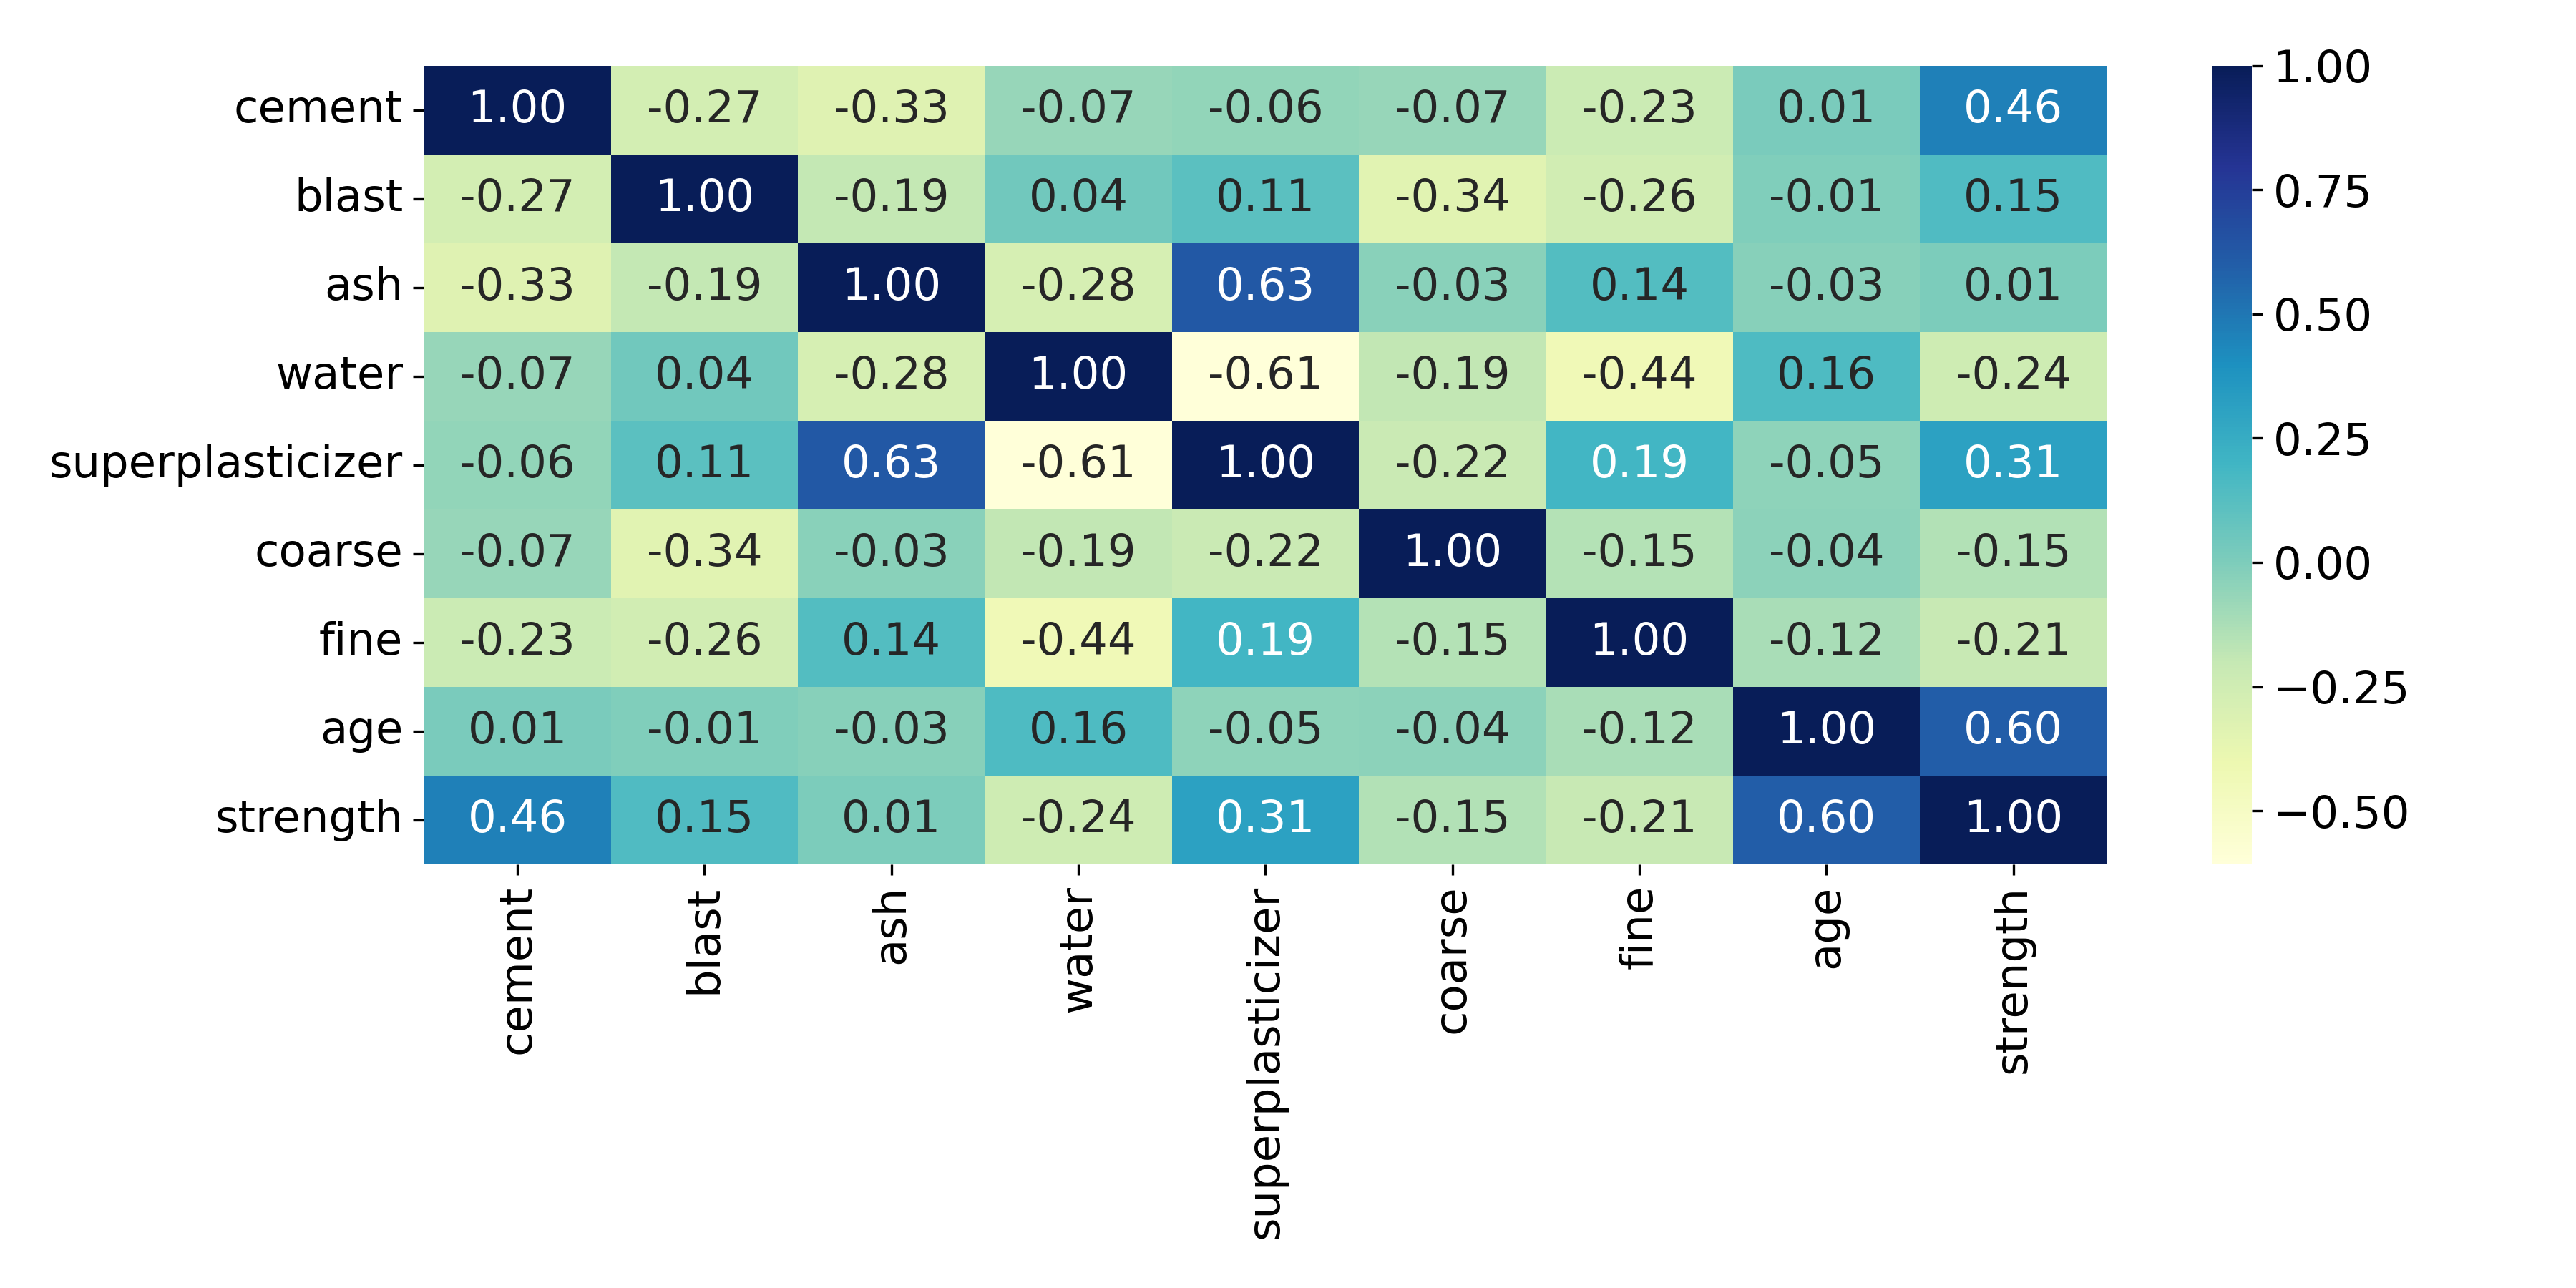
\includegraphics[width=1\textwidth]{../scripts/images/corr.png}
    Quelle: Eigene Darstellung, \ref{linreg}.
    \label{pic:corr}
\end{figure}

\section{Modellierung der linearen Regression}

Um die Beziehung zwischen den unabhängigen Variablen und der Zielvariablen  zu untersuchen, 
wurde ein lineares Regressionsmodell aufgestellt. 
Zur Bewertung der Vorhersageleistung des Modells und zur Vermeidung von Overfitting wurde der 
Datensatz in zwei Teile aufgeteilt: 80\% der Daten dienten als Trainingsset zur 
Anpassung des Modells, während die restlichen 20\% als Testset verwendet wurden, 
um die Modellleistung anhand neuer, unbekannter Daten zu evaluieren. 
Diese Aufteilung erfolgte zufällig, aber reproduzierbar, durch Festlegen eines Seed-Werts 
für den Zufallszahlengenerator, der eine konsistente Teilung des Datensatzes ermöglicht.

Das Trainingsset wurde dazu verwendet, die Koeffizienten der linearen Regression zu schätzen, 
die den Einfluss jeder unabhängigen Variablen auf die Zielvariable quantifizieren. 
Anschließend wurde das Modell mit dem Testset geprüft, um seine Vorhersagegenauigkeit zu bewerten. 
Die Leistung des Modells wurde anhand von Metriken wie dem mittleren quadratischen Fehler (Mean Squared Error, MSE) gemessen, 
die ein Maß für die Abweichung der Modellvorhersagen von den tatsächlichen Werten darstellen.

Codeauschnitt \ref{code:model} und \ref{code:model-train} zeigen das Trainieren und Testen der zugrundeliegenden Daten 
eines linearen Regressionsmodells:

\lstinputlisting[language=Python,label=code:model, firstline=35, lastline=53, 
    caption={Initialisierung eines linearen Regressionsmodells, \ref{linreg}.}, captionpos=top]{../scripts/linreg.py}


\lstinputlisting[language=Python,label=code:model-train, firstline=297, lastline=303, 
    caption={Training und Testen eines linearen Regressionsmodells, \ref{linreg}.}, captionpos=top]{../scripts/linreg.py}


\section{Berechnung von SHAP-Werten}

Um SHAP-Werte zu berechnen, wird zunächst ein SHAP-Explainer-Objekt erstellt. In diesem Fall wird der Explainer 
von SHAP mit dem trainierten linearen Regressionsmodell und dem Trainingsdatensatz initialisiert. 
Anschließend werden die SHAP-Werte für die Testdaten berechnet, um die Beiträge der einzelnen Merkmale 
zu analysieren. Der Typ des Explainers wird durch die Art des übergebenen Modells bestimmt. 
Da in diesem Beispiel ein lineares Modell verwendet wird, wird automatisch ein geeigneter Explainer 
für lineare Modelle ausgewählt.

Das folgende Codeausschnitt \ref{code:shap} zeigt die Initialisierung des SHAP-Explainers und die Berechnung der SHAP-Werte:

\lstinputlisting[language=Python,label=code:shap, firstline=309, lastline=310, 
    caption={Berechnung von SHAP-Werten für das lineare Regressionsmodell, \ref{linreg}.}, captionpos=top]{../scripts/linreg.py}

Das Explainer-Objekt enthält neben den SHAP-Werten (.values), 
die die Einflüsse der einzelnen Merkmale der Testmenge auf die Modellvorhersage quantifizieren, 
auch die Basiswerte (.base\_values), die die durchschnittliche Vorhersage des Modells darstellen, 
und die ursprünglichen Merkmalsausprägungen (.data), die für die Berechnung dieser Werte verwendet wurden \cite[S. 51]{Molnar_2023}.

Dies bildet die Grundlage für den nächsten entscheidenden Schritt: 
die Visualisierung und tiefere Analyse dieser Werte. Die SHAP-Bibliothek bietet eine 
Reihe von leistungsstarken Visualisierungswerkzeugen, die es ermöglichen, die Auswirkungen 
der einzelnen Merkmale auf die Modellvorhersagen intuitiv und verständlich abzubilden. 

Im folgenden Kapitel \ref{chapter:results} werden diese Visualisierungen im Detail vorgestellt. 
Anhand von Beeswarm-Plots, Dependence-Plots und Bar-Plots werden die Ergebnisse der 
SHAP-Analyse dargestellt, die ein umfassendes Bild der Einflüsse und Wichtigkeiten der 
verschiedenen Merkmale im Kontext des linearen Regressionsmodells bieten.

Die Grafiken wurden mithilfe der \textsf{shap}-Bibliothek wie folgt erzeugt:

\lstinputlisting[language=Python,label=code:img, firstline=92, lastline=129, 
    caption={Erzeugen der SHAP Plots, \ref{linreg}.}, captionpos=top]{../scripts/linreg.py}

